\chapter {Model builder and Subcircuit builder}\label{chap8}
\section {Model builder}



Spice based simulators include a feature which allow accurate modeling of semiconductor devices such as diodes, transistors etc. Oscad Model Builder provides a facility to define a new model for devices such as diodes, MOS, BJT, JFET, IGBT, Magnetic core etc. Model Builder in Oscad asks for the value of parameters depending on the type of the device for which a model is required. The parameter values can be obtained from a datasheet of the device. A newly created model can be exported to the model library and one can import it for different projects, whenever required. Model Builder also provides a facility to edit existing models. 

\subsection{Example}
Let us take an example of Bridge rectifier circuit containing diode model 1N4007 and see how Model Builder works in Oscad. Refer figure \ref{bridge-rectifier} for the Bridge rectifier circuit schematic.

\begin{figure}[t]%h stands for 'here'. If h is removed then the fig will go to the bottom or to the next page.
\begin{center}
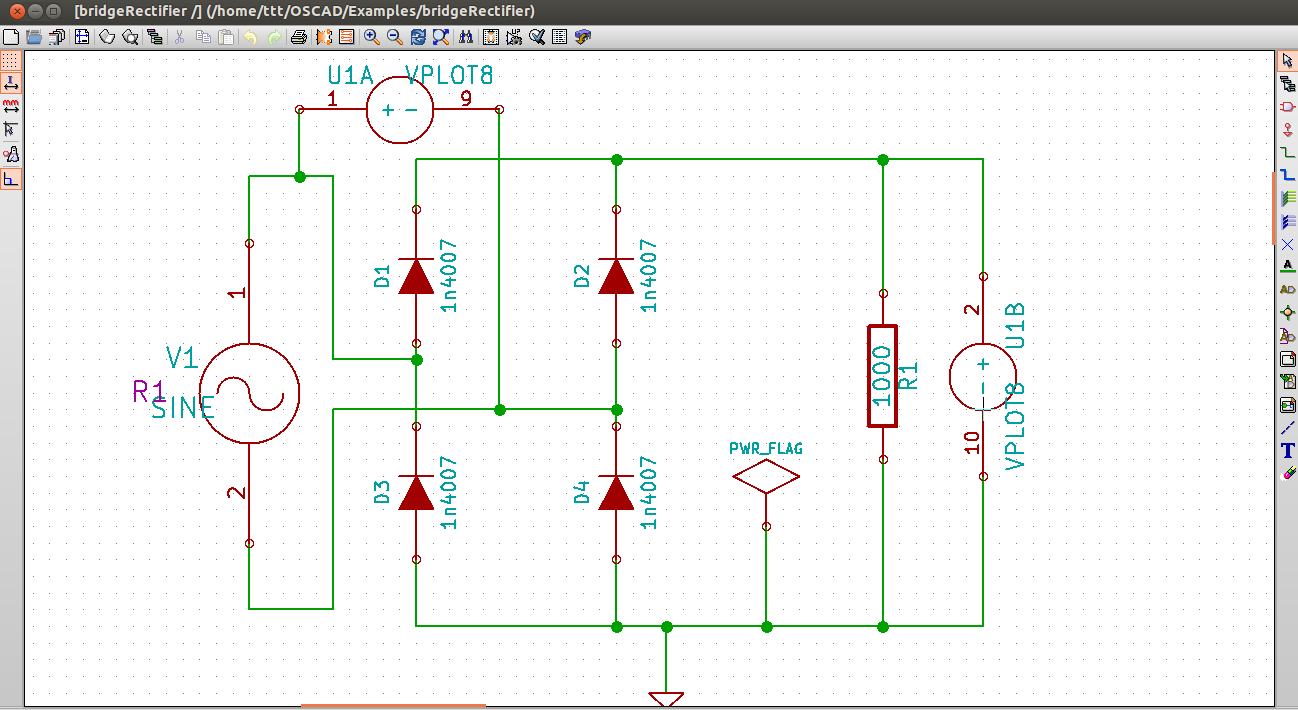
\includegraphics[width=1\linewidth]{figures/B-Rectifier-schematic.png}%If the fig is appearing too big/small, change the scaling factor 0.2
\caption{Bridge rectifier circuit schematic}
\label{bridge-rectifier}
\end{center}
\end{figure}

First create the circuit schematic of the Bridge Rectifier shown in figure \ref{bridge-rectifier} as explained in chapter \ref{chap5}. In this schematic, change reference field\index{reference field} of 1n4007 to ``D". Here reference field ``D" indicates that it is a diode model. Generate the spice netlist.

Now to build a new model for the diode 1N4007, click on the ``Model Builder" from the toolbar of Oscad. It opens up ``Model Select" window which shows 1N4007. Since we are going to create a new model, we will click on "cancel" button as shown in figure \ref{cancel}. Then click on ``New" from ``File" drop-down menu as shown in figure \ref{new}. An ``Ngspice Model Editor" window will open up. In the ``Enter Component name" field, type ``1N4007". In the "Enter type of Component" option, select ``Diode" and finally click on ``OK" button. This window is illustrated in figure \ref{select}. Then you will get a window where it asks for the value of model parameters for diode 1N4008 such as reverse breakdown voltage (BV), ohmic resistance (RS) etc. as shown in Figure \ref{edit}. Here you can change the values of the model parameters for 1N4007 diode model as it is given in the datasheet and then click on “OK” button to save it.


\begin{figure}[t]%h stands for 'here'. If h is removed then the fig will go to the bottom or to the next page.
\begin{center}
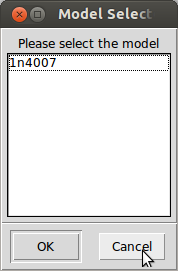
\includegraphics[width=0.3\linewidth]{figures/cancel-model-b.png}%If the fig is appearing too big/small, change the scaling factor 0.2
\caption{Cancel selecting existing model}
\label{cancel}
\end{center}
\end{figure} 

\begin{figure}[t]%h stands for 'here'. If h is removed then the fig will go to the bottom or to the next page.
\begin{center}
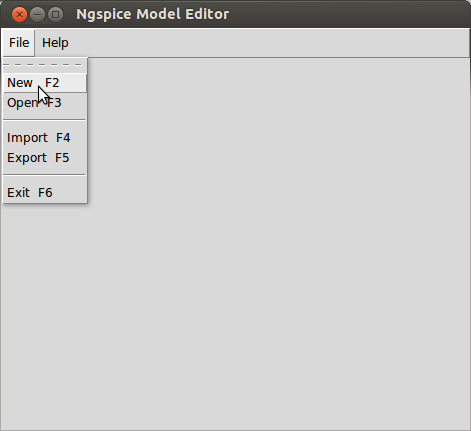
\includegraphics[width=0.4\linewidth]{figures/new-model-0.png}%If the fig is appearing too big/small, change the scaling factor 0.2
\caption{Select new Model}
\label{new}
\end{center}
\end{figure} 

\begin{figure}[t]%h stands for 'here'. If h is removed then the fig will go to the bottom or to the next page.
\begin{center}
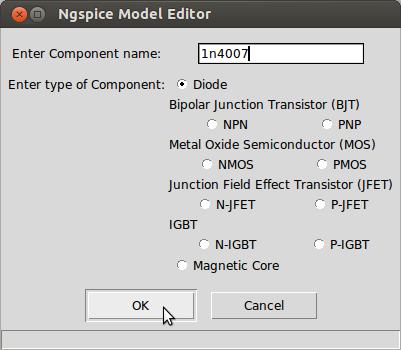
\includegraphics[width=0.8\linewidth]{figures/select-mod-type.png}%If the fig is appearing too big/small, change the scaling factor 0.2
\caption{Select type of model}
\label{select}
\end{center}
\end{figure} 

\begin{figure}[t]%h stands for 'here'. If h is removed then the fig will go to the bottom or to the next page.
\begin{center}
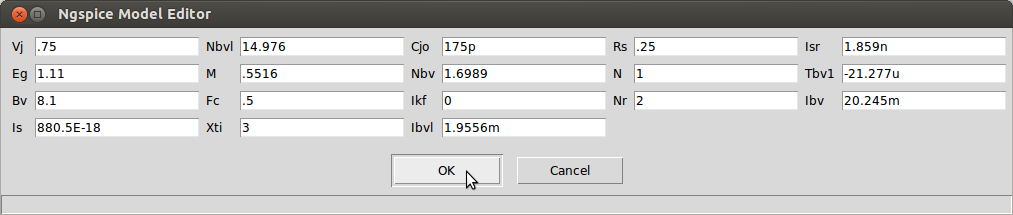
\includegraphics[width=1\linewidth]{figures/model-parameters.png}%If the fig is appearing too big/small, change the scaling factor 0.2
\caption{Edit model paramters}
\label{edit}
\end{center}
\end{figure}

Once a new diode model of 1n4007 is created it can be exported to the model library\index{model library} as shown in the Figure \ref{export}. Whenever required, one can also import it for different projects as shown in the figure \ref{import-1} and \ref{import-2}.

\begin{figure}[t]%h stands for 'here'. If h is removed then the fig will go to the bottom or to the next page.
\begin{center}
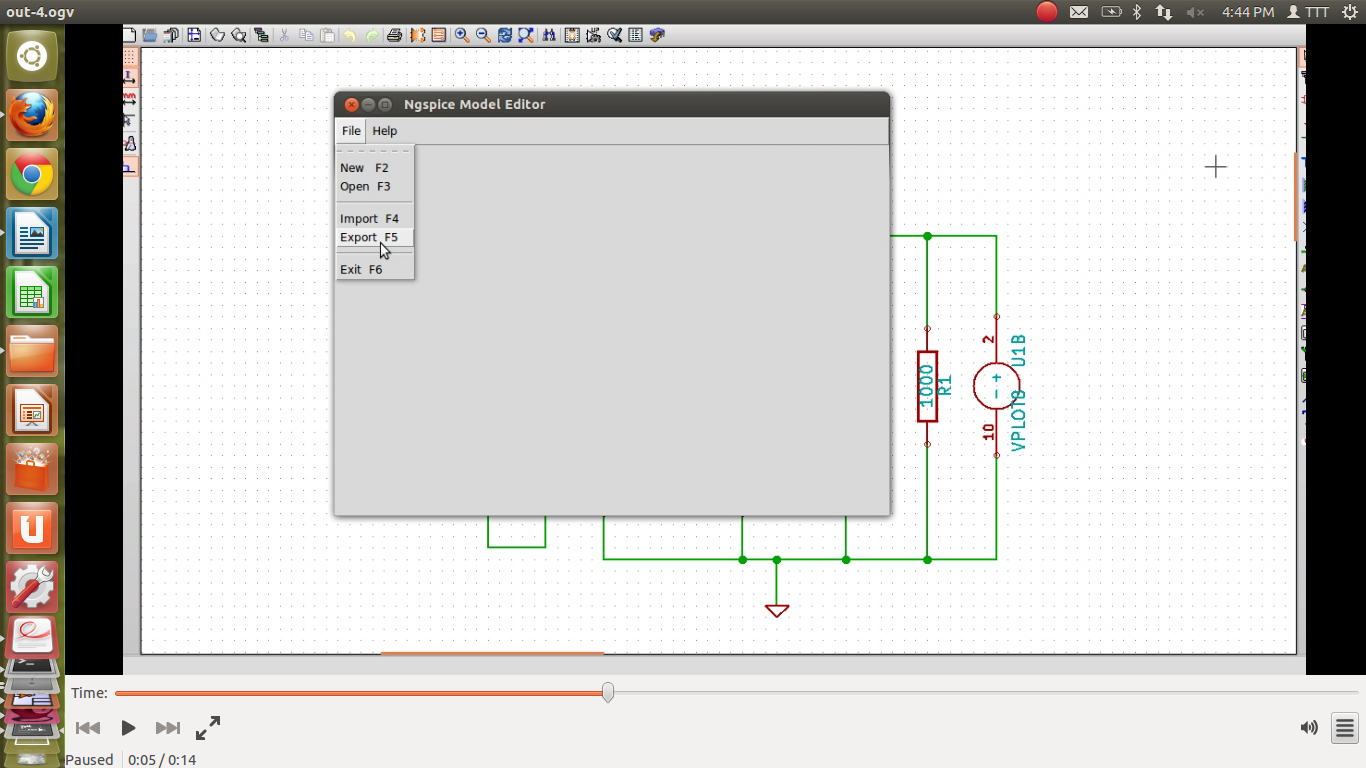
\includegraphics[width=0.6\linewidth]{figures/model-build-export.png}%If the fig is appearing too big/small, change the scaling factor 0.2
\caption{Export model}
\label{export}
\end{center}
\end{figure}

\begin{figure}[t]%h stands for 'here'. If h is removed then the fig will go to the bottom or to the next page.
\begin{center}
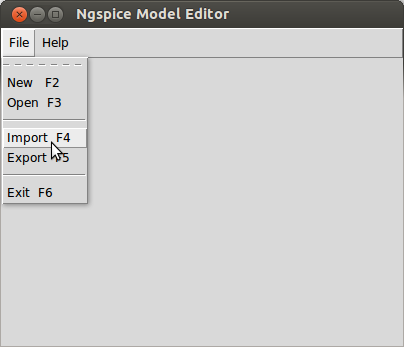
\includegraphics[width=0.5\linewidth]{figures/import-0.png}%If the fig is appearing too big/small, change the scaling factor 0.2
\caption{Import model-1}
\label{import-1}
\end{center}
\end{figure}

\begin{figure}[t]%h stands for 'here'. If h is removed then the fig will go to the bottom or to the next page.
\begin{center}
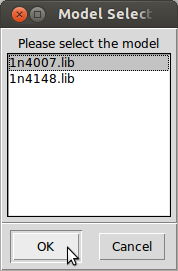
\includegraphics[width=.3\linewidth]{figures/import-mod.png}%If the fig is appearing too big/small, change the scaling factor 0.2
\caption{Import model-2}
\label{import-2}
\end{center}
\end{figure}


\section {Subcircuit Builder}
Subcircuit is a way to implement hierarchical modeling\index{hierarchical modeling}. Once a subcircuit for a component is created, it can be used for different circuits. Oscad provides an easy way to create a subcircuit in steps. 

\subsection{Example}

Let us take an example of building a subcircuit of IC 555 timer which is a part of Astable Multivibrator circuit.

Create the schematic of the Astable multivibrator as shown in the figure \ref{LM555N}. Before making the subcircuit for components, make sure that the ``Reference Field" of these component should always be ``X". Let us see how to change ``Reference Field"  of a component. Right click on U? of the LM555N IC and choose ``Field Reference". This is shown in figure \ref{555-field-ref}. Then choose ``Edit field" as shown in figure \ref{555-edit-field}. Change the reference field of LM555N from U? to X. Here the reference field X denotes that LM555N can have a subcircuit. This is shown in figure \ref{555-ref-change}

\begin{figure}[t]%h stands for 'here'. If h is removed then the fig will go to the bottom or to the next page.
\begin{center}
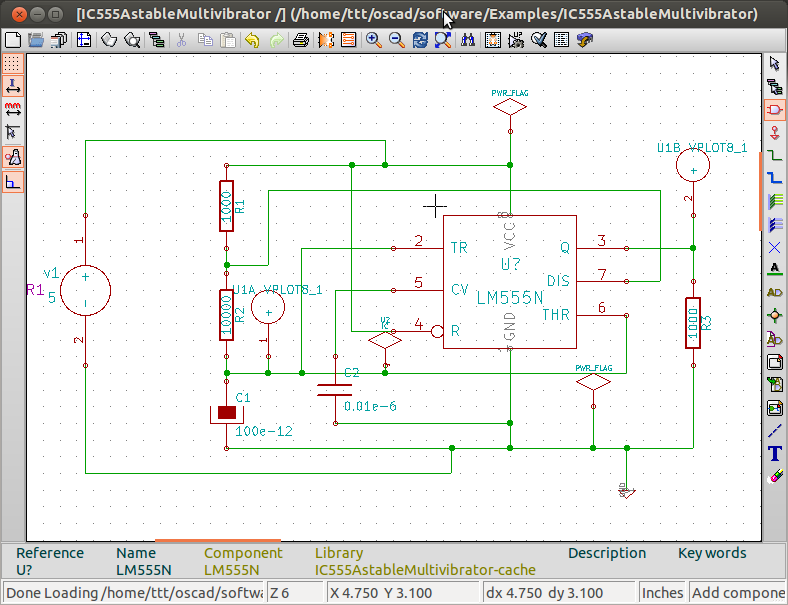
\includegraphics[width=1\linewidth]{figures/555-schematic.png}%If the fig is appearing too big/small, change the scaling factor 0.2
\caption{Astable multivibrator circuit Schematic}
\label{LM555N}
\end{center}
\end{figure}


\begin{figure}[t]%h stands for 'here'. If h is removed then the fig will go to the bottom or to the next page.
\begin{center}
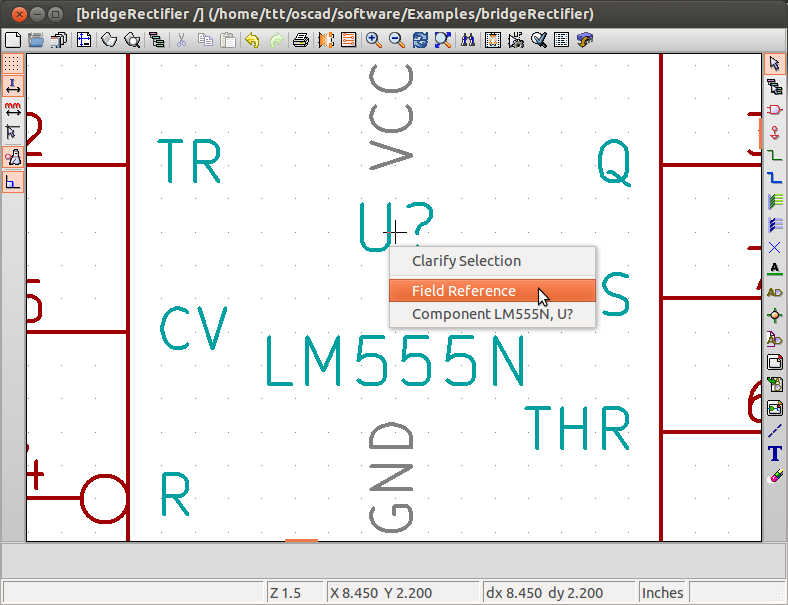
\includegraphics[width=1\linewidth]{figures/555-field-ref.png}%If the fig is appearing too big/small, change the scaling factor 0.2
\caption{Choosing field reference of LM555N}
\label{555-field-ref}
\end{center}
\end{figure}

\begin{figure}[t]%h stands for 'here'. If h is removed then the fig will go to the bottom or to the next page.
\begin{center}
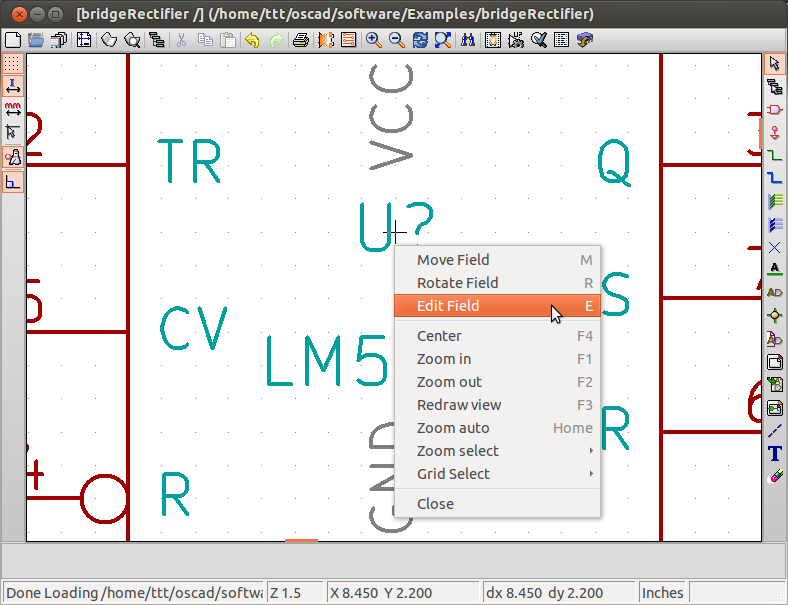
\includegraphics[width=1\linewidth]{figures/555-edit-field.png}%If the fig is appearing too big/small, change the scaling factor 0.2
\caption{Choosing Edit field of LM555N}
\label{555-edit-field}
\end{center}
\end{figure}


\begin{figure}[t]%h stands for 'here'. If h is removed then the fig will go to the bottom or to the next page.
\begin{center}
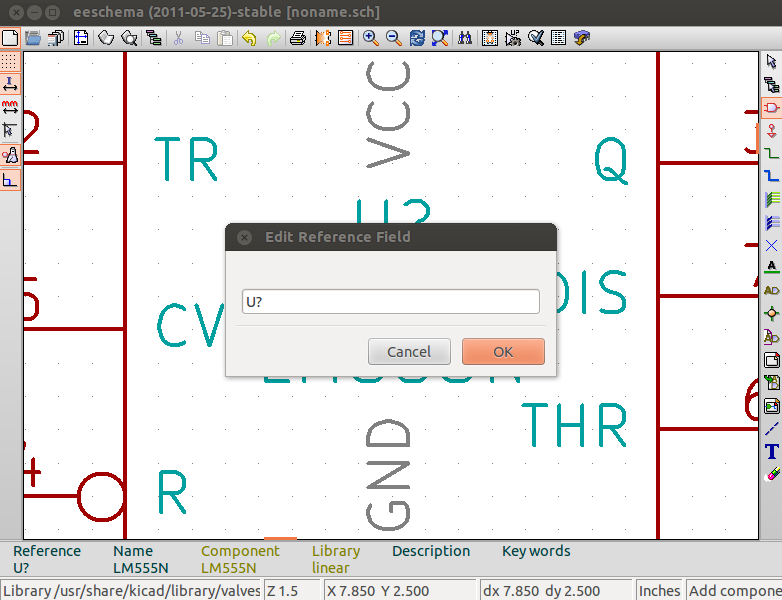
\includegraphics[width=1\linewidth]{figures/555-ref-change.png}%If the fig is appearing too big/small, change the scaling factor 0.2
\caption{Changing reference field of LM555N from U? to X}
\label{555-ref-change}
\end{center}
\end{figure}


Now to create Subcircuit, click on the “Sub Circuit Builder” option from the Tool bar of Oscad. You will get a window displaying the list of ``Field Values" of components whose ``Reference Field" value is ``X". It is shown in Figure \ref{sub-sel}.


\begin{figure}[t]%h stands for 'here'. If h is removed then the fig will go to the bottom or to the next page.
\begin{center}
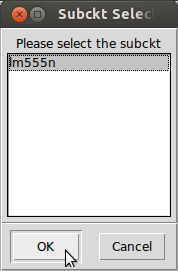
\includegraphics[width=0.3\linewidth]{figures/select-subckt.png}%If the fig is appearing too big/small, change the scaling factor 0.2
\caption{Select Model}
\label{sub-sel}
\end{center}
\end{figure}


Once you select the subcircuit it opens up the Schematic Editor where you can draw the schematic of the subcircuit. After you finish creating the subcircuit, connect a port to the external pins of the subcircuit. Port can be found under the ``Place a component" option. The subcircuit of LM555N is shown in Figure \ref{555}. Once you completed the creation of the subcircuit save it in the respective project folder and close the Schematic editor. 

\begin{figure}[t]%h stands for 'here'. If h is removed then the fig will go to the bottom or to the next page.
\begin{center}
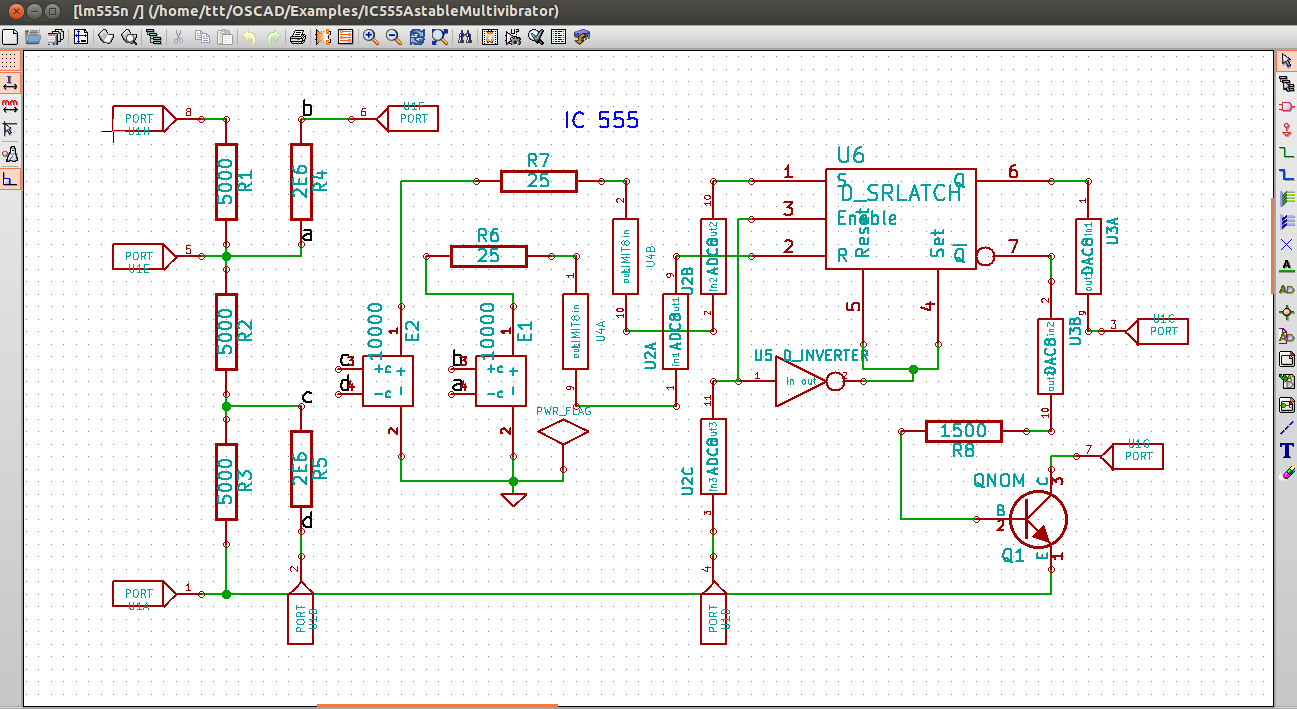
\includegraphics[width=1\linewidth]{figures/subcircuit.png}%If the fig is appearing too big/small, change the scaling factor 0.2
\caption{IC 555 timer subcircuit}
\label{555}
\end{center}
\end{figure}

When you close the Schematic Editor, a terminal window will pop-up. It will ask you to enter the value for the different parameters of subcircuit as shown in the Figure \ref{para}.

\begin{figure}[t]%h stands for 'here'. If h is removed then the fig will go to the bottom or to the next page.
\begin{center}
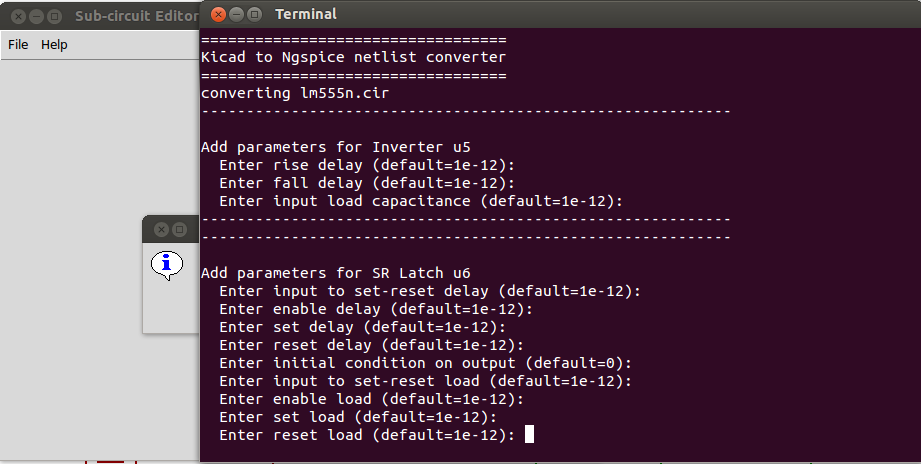
\includegraphics[width=1\linewidth]{figures/subcircuit-parameters.png}%If the fig is appearing too big/small, change the scaling factor 0.2
\caption{IC 555 timer subcircuit - parameters}
\label{para}
\end{center}
\end{figure}

At the end of the terminal, after you entered all the parameters, you will see the message: \\{\tt The ngspice netlist has been written in lm555n.cir.out\\
The scilab netlist has been written in lm555n.cir.ckt.\\
Press Enter to quit}\\ 
This message means that netlist for the subcircuit is created. It is shown in the Figure \ref{net}.

\begin{figure}[t]%h stands for 'here'. If h is removed then the fig will go to the bottom or to the next page.
\begin{center}
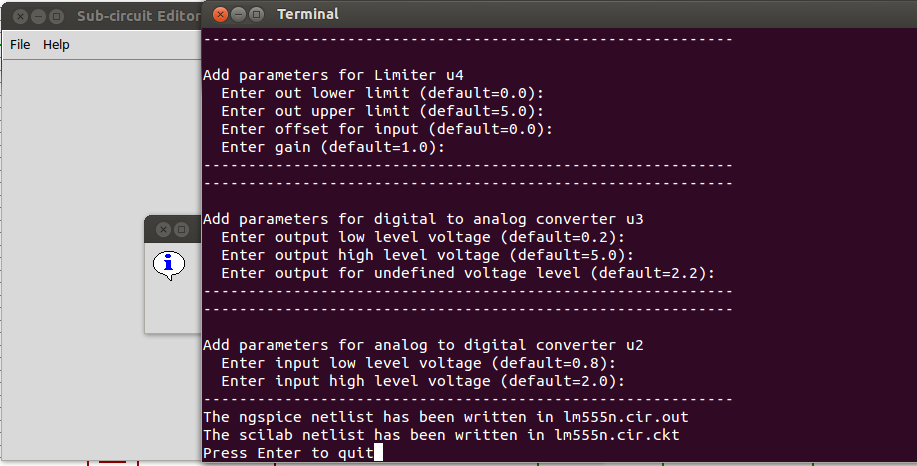
\includegraphics[width=1\linewidth]{figures/netlist-generation.png}%If the fig is appearing too big/small, change the scaling factor 0.2
\caption{Netlist conversion}
\label{net}
\end{center}
\end{figure}

Finally it gives a pop-up saying ``Created subcircuit lm555n.sub". It is shown in figure \ref{done}. Click on OK. This completes the subcircuit creation. 

\begin{figure}[t]%h stands for 'here'. If h is removed then the fig will go to the bottom or to the next page.
\begin{center}
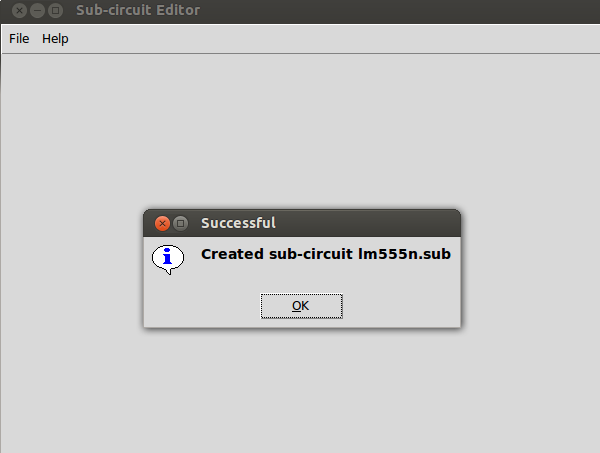
\includegraphics[width=0.5\linewidth]{figures/subcircuit-created.png}%If the fig is appearing too big/small, change the scaling factor 0.2
\caption{Subcircuit creation successfull}
\label{done}
\end{center}
\end{figure}

Once subcircuit is created, it can be exported to the subcircuit library as shown in Figure \ref{exp} and whenever required one can import it for different projects as shown in the figure \ref{import}.

\begin{figure}[t]%h stands for 'here'. If h is removed then the fig will go to the bottom or to the next page.
\begin{center}
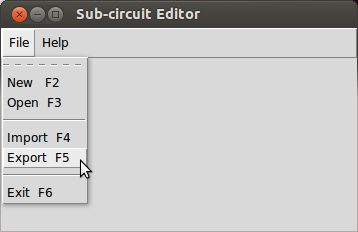
\includegraphics[width=0.5\linewidth]{figures/export-subcircuit.png}%If the fig is appearing too big/small, change the scaling factor 0.2
\caption{Export Subcircuit}
\label{exp}
\end{center}
\end{figure}

\begin{figure}[t]%h stands for 'here'. If h is removed then the fig will go to the bottom or to the next page.
\begin{center}
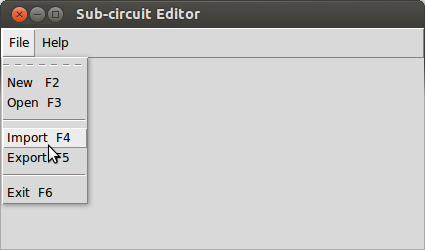
\includegraphics[width=0.5\linewidth]{figures/import-subckt.png}%If the fig is appearing too big/small, change the scaling factor 0.2
\caption{Import Subcircuit}
\label{import}
\end{center}
\end{figure}

Finally close the subcircuit editor window.









